
\documentclass[letterpaper,12pt]{article}
\usepackage[english]{babel}
\usepackage[utf8x]{inputenc}
\usepackage{amsmath}
\usepackage[paper=letterpaper,left=25mm,right=25mm,top=25mm,bottom=25mm]{geometry}
\usepackage{graphicx}
\usepackage[colorinlistoftodos]{todonotes}
\usepackage{newtxtext,newtxmath}
\usepackage{enumitem}
\usepackage{bm}
\usepackage{hyperref}
\usepackage{xfrac}
\usepackage{multirow}
\usepackage{subcaption}

% Replace regular l with \ell
\mathcode`l="8000
\begingroup
\makeatletter
\lccode`\~=`\l
\DeclareMathSymbol{\lsb@l}{\mathalpha}{letters}{`l}
\lowercase{\gdef~{\ifnum\the\mathgroup=\m@ne \ell \else \lsb@l \fi}}%
\endgroup

\begin{document}
	
\begin{titlepage}
	
	\newcommand{\HRule}{\rule{\linewidth}{0.5mm}}
	
	\center
	
	\textsc{\LARGE University of British Columbia}\\[1.5cm]
	\textsc{\Large MECH 325 - Mechanical Design I}\\[0.5cm]
	\textsc{\Large Assignment 3}\\[0.5cm]
	
	\HRule \\[0.8cm]
	{ \huge \bfseries Bearings, Shaft Accessories, Fasteners}\\[0.4cm]
	\HRule \\[1cm]
	
	{\Large GROUP C2}\\
	\vspace{0.5cm}
	
	\begin{minipage}{0.4\textwidth}
		\begin{flushleft} \large
			\emph{Team Member:}\\
			Kota Chang\\
			Chuan Du\\
			Donney Fan\\
			Dvir Hilu\\
			Michael Ko\\
			Priyansh Malik\\
			Darren Tong\\
		\end{flushleft}
	\end{minipage}
	~
	\begin{minipage}{0.4\textwidth}
		\begin{flushright} \large
			\emph{Student Number:} \\
			12345678\\
			12345678\\
			12345678\\
			12345678\\
			12345678\\
			12345678\\
			24711137
			
		\end{flushright}
	\end{minipage}\\[2cm]
	
	{\large \today}\\[2cm]
	
	{\Large\textbf{
		Performance Metric: 0.00187$\text{ [kg}\cdot\text{\$]}^{-1}$
	}}
	
	%\includegraphics{logo.png}\\[1cm]
	
	\vfill % Fill the rest of the page with whitespace
	
\end{titlepage}

\section{Summary}

\subsection{Introduction}
This document presents the design process of selecting and positioning bearings, shaft accessories, and bolts for the candy polishing machine, the ClumpBuster-2000. Since our design utilizes an idler shaft, the bearing and shaft accessory analysis was done on both the idler and tumbler shafts. Moreover, bolt stress calculations were performed to ensure a secure connection to the motor mount.

\subsection{Final Performance Results}
\vspace{4mm}
\begin{center}
	\begin{tabular}{ |p{4cm}||p{2cm}|p{8cm}|  }
		\hline
		\textbf{Item} & \textbf{Cost (\$)} & \textbf{Description} \\
		\hline
		\hline
		\textbf{Tumbler Drum Shaft} & & \\
		Stock Shaft & 34.62 & Stock diameter of 35 mm (1045 Carbon Steel)\\
		Machining & 10.84 & Reduce to 34.93 mm and to 30 mm for bearings\\
		Bearing 1 & 60.00 & 02-30 Series Cylindrical Roller Bearing \\
		Bearing 2 & 60.00 & 02-30 Series Deep Grove Ball Bearing \\
		Retaining Ring Groove & 20.00 & Groove to support Bearing 2\\
		\hline
		\hline
		\textbf{Motor Mount} & & \\
		Bolt-Nut Pair (x4) & 28.00 & SAE Grade No. 5 Steel Bolts, Size 1" \\
		 & & Regular Hexagonal Nut, Nominal Size 1" \\
		\hline
		\hline
		\textbf{Total} & \textbf{213.46}& - \\
		\hline
	\end{tabular}
\end{center}
\noindent The total mass of the Tumbler Drum Shaft was calculated to be: filler kg.

\subsection{Approach \& Methods}
Our primary focus for this design was to satisfy safety factor requirements first as it was important for our team to ensure that our proposed design would be mechanically sound for this operation. We would then optimize the cost and performance of our system. Equilibrium moment and force calculations were used to identify the ideal location for bearing placements, while comprehensive stress calculations were performed to select the required bolts and nuts.
\\\\
The following assumptions were made in the our design:
\begin{itemize}
    \itemsep0em
    \item Shaft deflection has no effect on our bearing and shaft accessory placement calculations.
    \item Cost calculations and shaft accessory placements are not required for the idler shaft.
    \item Only the bending moment in the side-view plane shown in the assignment figure needs to be considered for bolt stress calculations.
    \item The loading on the bolts is cyclic due to the running operation of the ClumpBuster-2000.
    \item The height of the motor mount (25'') was decided on by assuming an operator would use the tumbling machine at chest-height.
    \item The top motor mounting plate is 8" x 8". Upper and lower plates are made of steel.
    \item The washers used for the bolts are also made out of steel, so for the stiffness calculations we assume the entire member configuration is made of the same material and thus can be treated as one uniform member.
    \item m There is sufficient space for the bolt to protrude the bottom of the plate to allow for the nut to be placed on and therefore a screw length of 2.5” (greater than the thickness of the plate) is satisfactory =
\end{itemize}

\subsection{ClumpBuster-2000 System Overview}
Below is an side-profile overview of the completed ClumpBuster-2000 System, with bearings, shaft accessories, and bolt placement locations. To focus on the locations of the sprockets, bearings, and retaining rings on the tumbler shaft, the chain belts were not included in the final drawing. On the upper tumbler shaft, there is a cylindrical roller bearing on the left, a deep groove bearing on the right flanking the shoulders, and a single retaining ring to constrain the deep groove bearing. See section 2.1.1.

\begin{figure}[!h]
\centering
  \begin{subfigure}[b]{0.45\textwidth}
    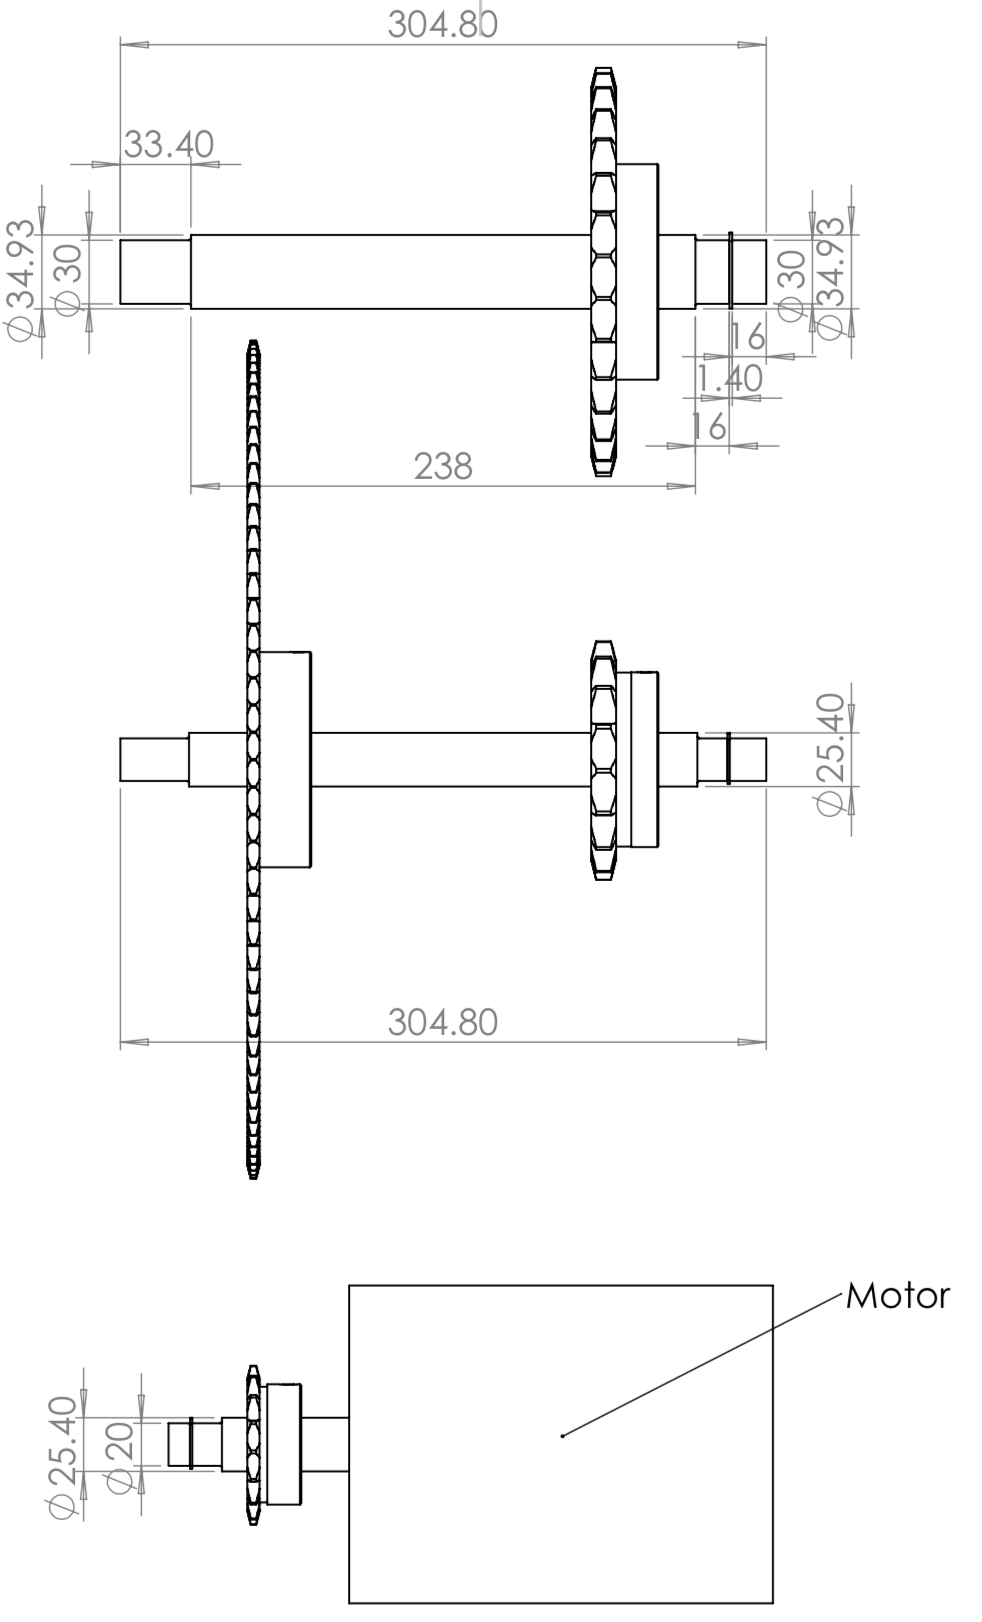
\includegraphics[width=8cm]{A3/shaft_drawing.png}
    \caption{Shaft Accessories Design}
    \label{fig:1}
  \end{subfigure}
  %
  \begin{subfigure}[b]{0.45\textwidth}
    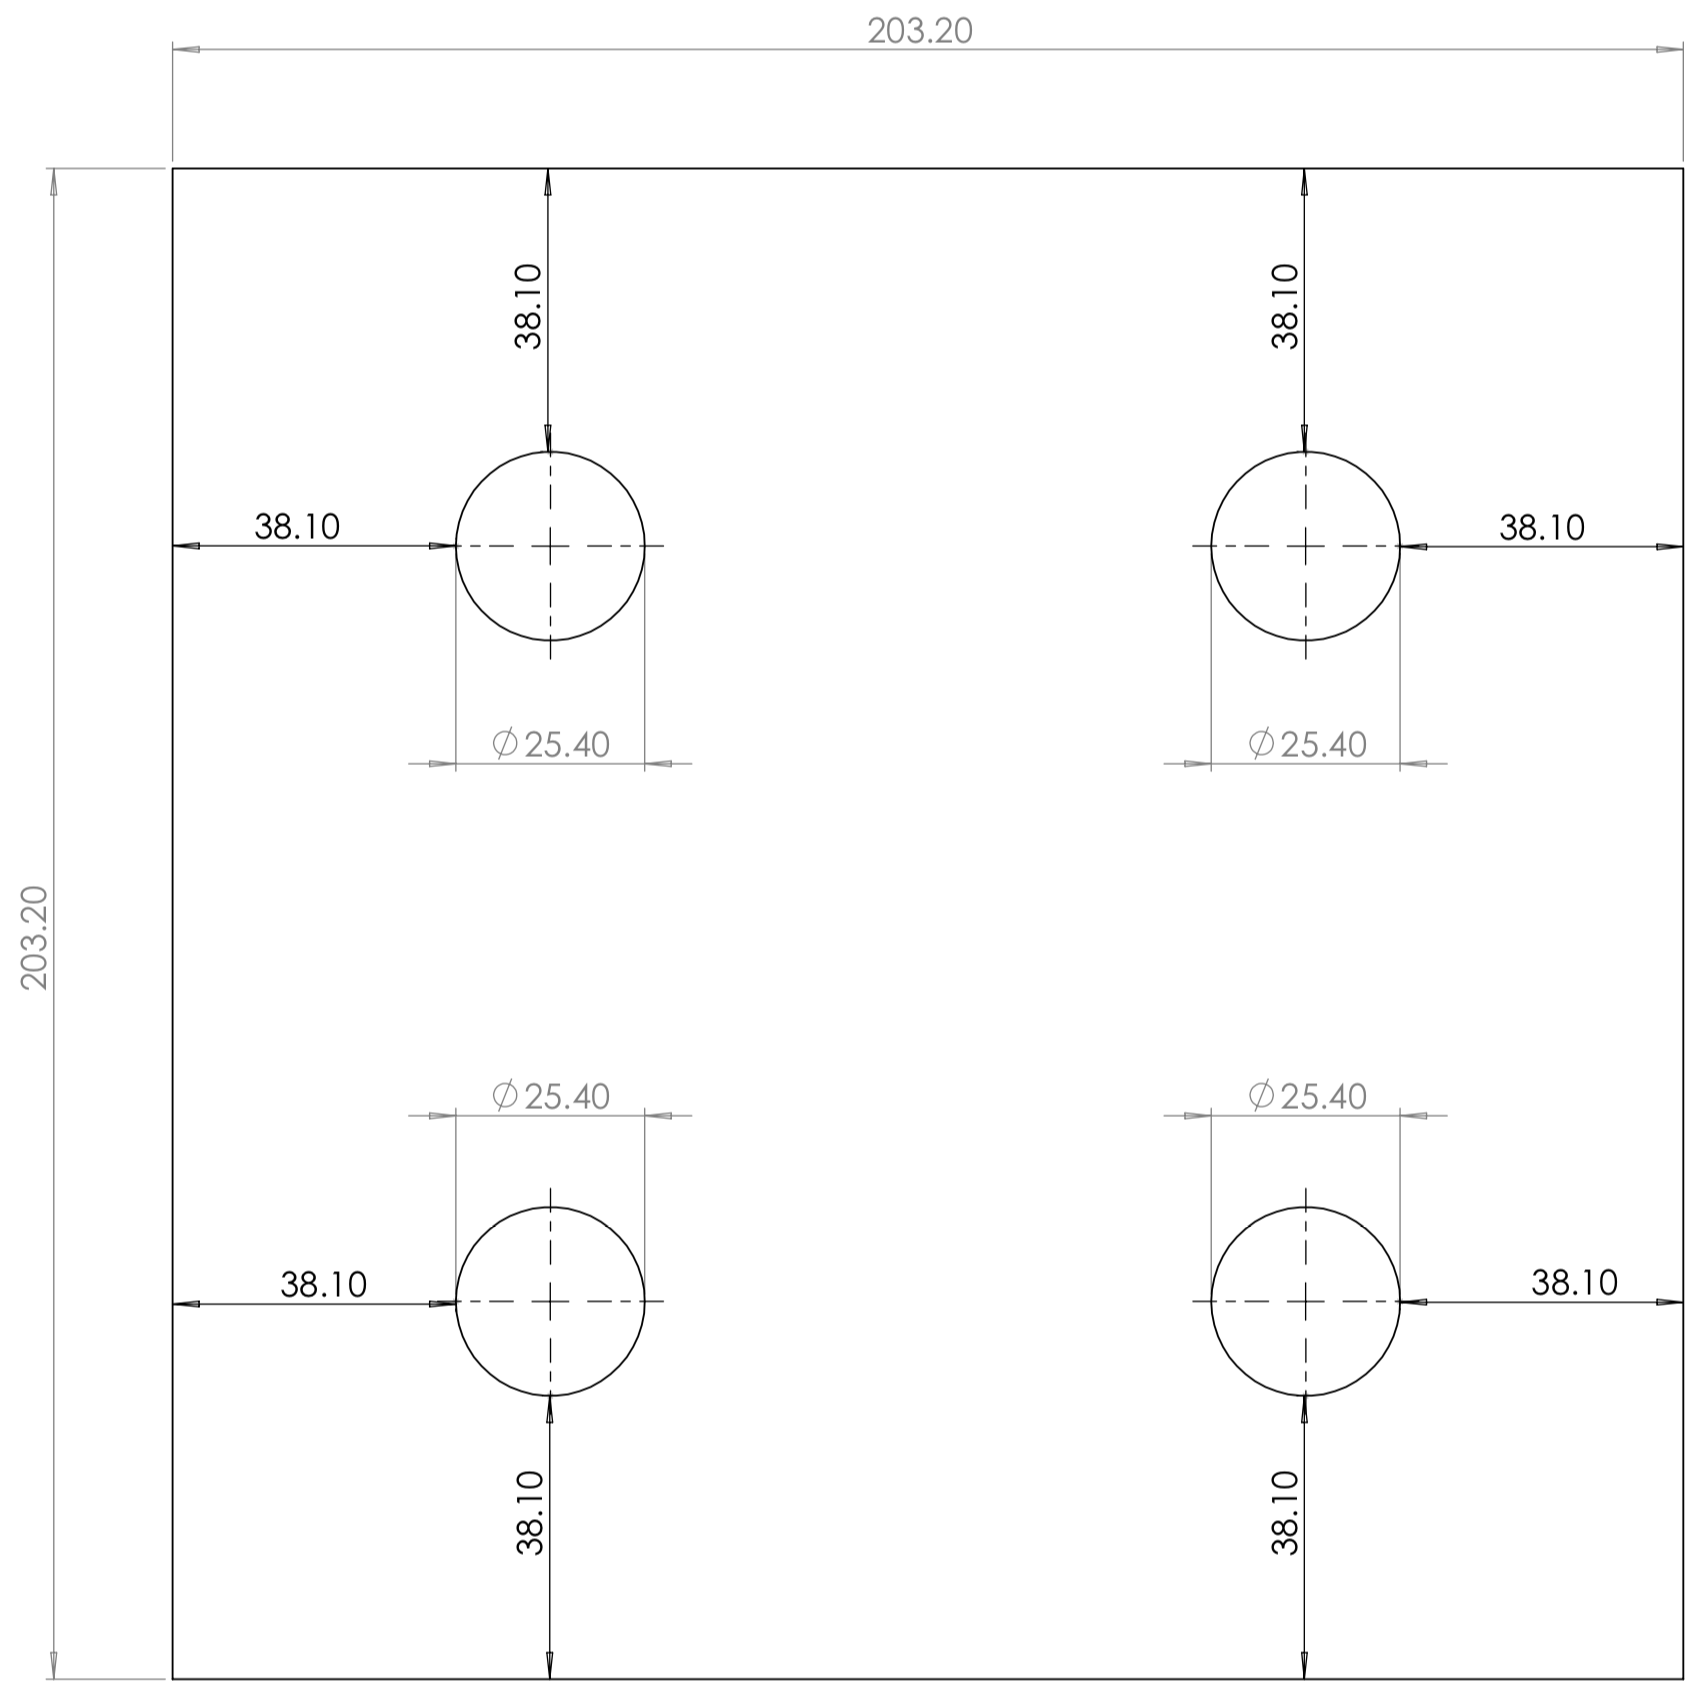
\includegraphics[width=8cm]{A3/mount_drawing.png}
    \caption{Motor Mount Design}
    \label{fig:2}
  \end{subfigure}
\end{figure}

\newpage

\section{Appendix}
\subsection{Shaft Design}
The objective of this section is to analyze the force and moment on the upper shaft and specify appropriate bearings to support the radial and axial load of the system. Selection of components involved careful consideration of various constraints such as available sprockets and bearing bore diameters. Selection was an iterative process and we will show sample analyses and results here.

\subsubsection{Force and Moment Analysis}
The sprocket on the upper shaft has a 34.93 mm bore width. We chose to purchase a stock shaft of 304.8 mm with a 35 mm diameter. Each end of the shaft is press-fit with a bearing suitable for the axial and radial load determined through static analysis. Since the drum is tilted at $30^{\circ} $, the bearings must support an axial load from mass of the system as well as jolting from the drum in operation. 

\begin{figure}[h]
    \centering
    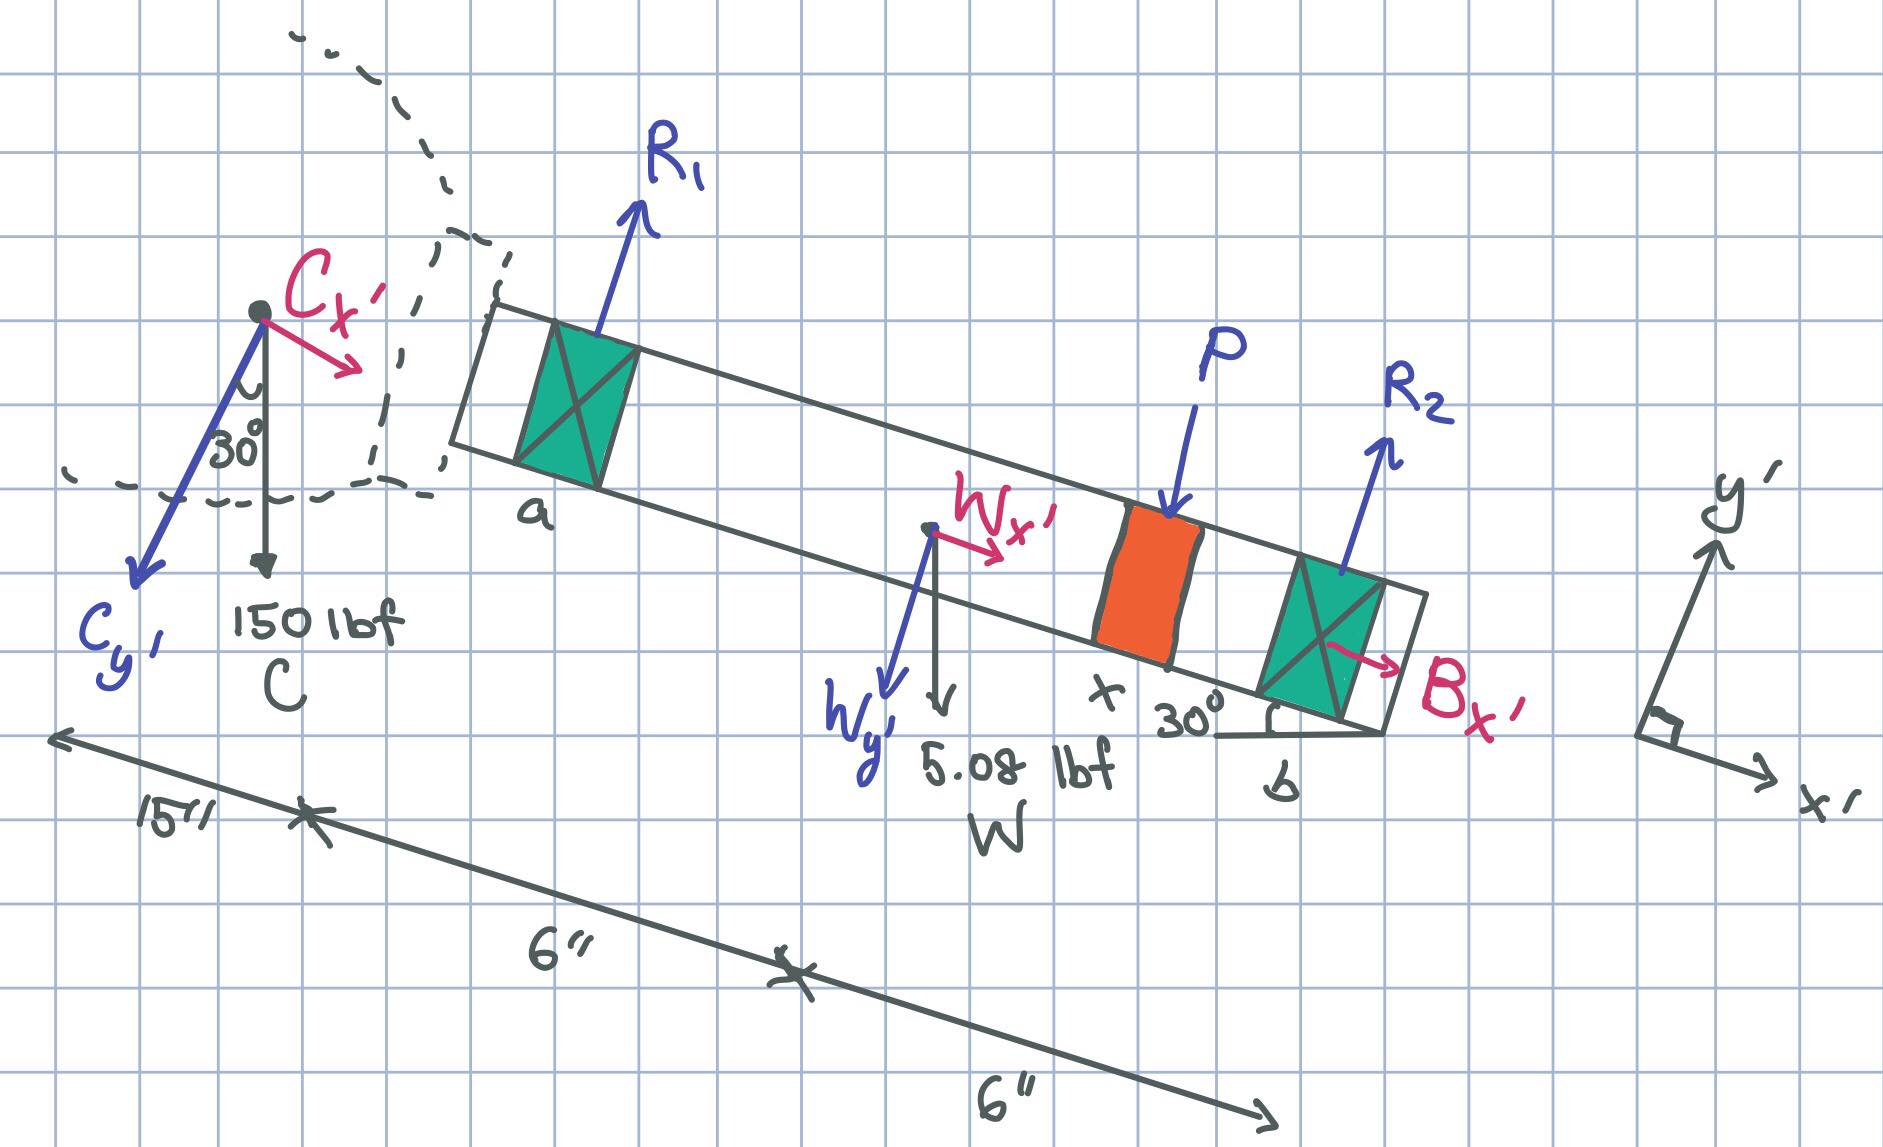
\includegraphics[width=10cm]{A3/MECH325A3FBD.jpg}
    \caption{Upper shaft free body diagram}
\end{figure}
    
\noindent The following static analysis are computed in imperial units.\\
The mass of the shaft is computed and projected in the tangential and normal directions.
\[ \begin{array}{lll}%
 W = \rho \pi r^2 L = 5.08 \text{ lbf} &  W_{x'} = W\sin{30^\circ}  &  W_{y'} = W\cos{30^\circ}\\
C = 150 \text{ lbf} &  C_{x'} = C\sin{30^\circ} &  C_{y'} = C\cos{30^\circ}\\
\end{array}\]%
Balance moments and forces in $x$ and $y$ directions,
\[ \begin{array}{lll}%
 \sum F_x = 0 = C_{x'} + W_{x'} - B_{x} &\Rightarrow& B_{x} = 77.544 \text{ lbf}\\
 \sum F_y = 0 = -C_{y'} + R_1 - W_{y'} - P - R_2 &\Rightarrow& R_1 = R_2 + 253.94\\
 \sum M_{A} = 0 = 16C_{y'} - 5W_{y'} - P(x-1) + 10R_2 &\Rightarrow& R_2 = 217.27 - 11.963x
\end{array}\]%

\noindent We choose to maximize the distance $x$ (distance of sprocket from the the bearing at $A$) to minimize $R_1$ and $R_2$. Letting $x = 10$ inches, we solve simultaneously and we have our results below in terms of magnitudes:

\begin{center}
	\begin{tabular}{ |p{1.5cm}||p{1.5cm}|p{2cm}|p{7cm}|  }
		\hline
		Symbol & Value & Units & Description\\
		\hline
		$\rho$ & 0.284 & lbf/in$^3$ & density of carbon steel\\
	    $L$ & 12 & in & length of shaft\\
		\hline
		$W$ & 5.08 & lbf  & drum shaft mass: 12" long 1.5" diameter\\
		%$W_{x'}$ & 2.54 & lbf  & drum shaft mass, tangent to shaft\\
		%$W_{y'}$ & 4.40 & lbf  & drum shaft mass, normal to shaft\\
        $C$ & 150 & lbf & jelly bean and drum mass\\
        %$C_{x'}$ & 75 & lbf  & jelly bean and drum mass, tangent to shaft\\	
		%$C_{y'}$ & 129.90 & lbf  & jelly bean and drum mass, normal to shaft\\
		$P$ & 119.63 & lbf  & intermediate to drum shaft chain force\\
		\hline
		$a$ & 1 & in  & distance from left end to left bearing\\
		$b$ & 11 & in  & distance from left end to right bearing\\
		$x$ & 10 & in  & distance from left end to sprocket \\
		\hline
		$R_1$ & 351.91 & lbf  & reaction at left bearing\\
		$R_2$ & 97.98 & lbf  & reaction at right bearing\\
		\hline
	\end{tabular}
\end{center}

\subsubsection{Force and Moment Diagrams}
Torque is transmitted between the drum and upper sprocket. The shear force is computed using method of virtual cuts and the moment diagram is obtained by the integral of the shear force diagram. 
%\begin{figure}[!htb]
%\minipage{0.32\textwidth}
%  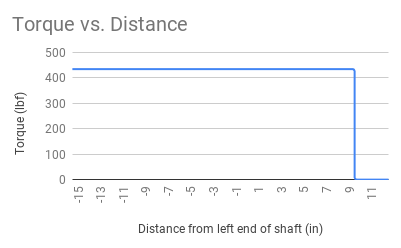
\includegraphics[width=\linewidth]{A3/torque_diagram.png}
%\endminipage\hfill
%\minipage{0.32\textwidth}
%  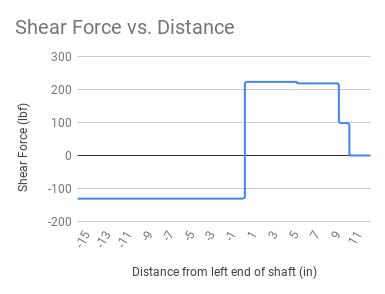
\includegraphics[width=\linewidth]{A3/shear_force_diagram.png}
%\endminipage\hfill
%\minipage{0.32\textwidth}%
%  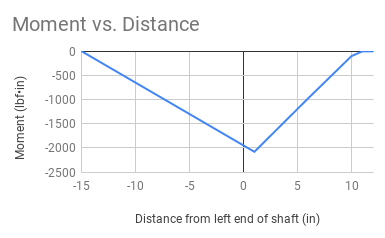
\includegraphics[width=\linewidth]{A3/moment_diagram.png}

%\endminipage
%\end{figure}

\begin{figure}[!h]
\centering
    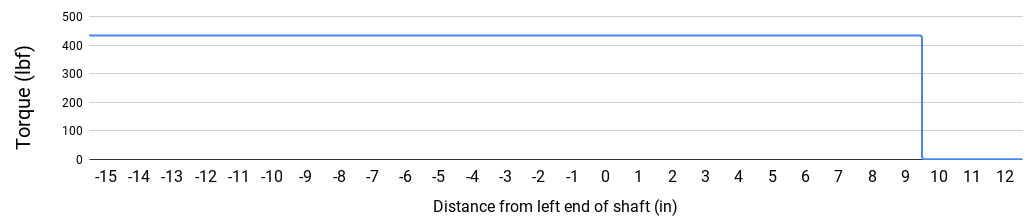
\includegraphics[width=\linewidth]{A3/torque_wide.png}
    \caption{Torque vs Distance on shaft}
\end{figure}
\vspace{-5mm}
\begin{figure}[!h]
\centering
    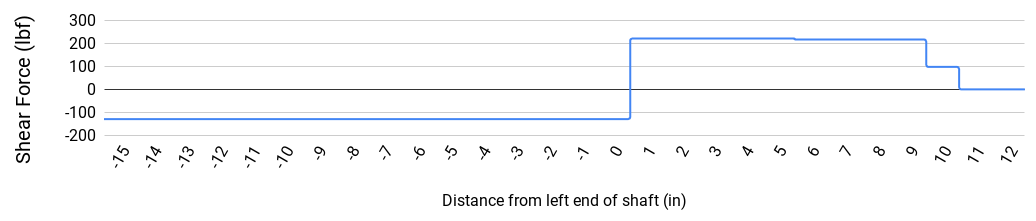
\includegraphics[width=\linewidth]{A3/shear_wide.png}
    \caption{Shear vs Distance on shaft}
\end{figure}
\vspace{-5mm}
\begin{figure}[!h]
\centering
    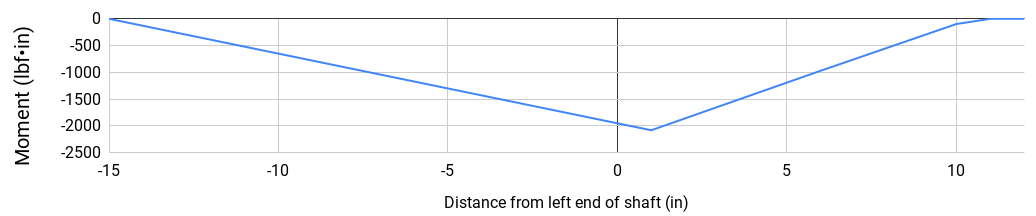
\includegraphics[width=\linewidth]{A3/moment_wide.png}
     \caption{Moment vs Distance on shaft}
\end{figure}

\subsubsection{Material Properties}

We selected 1045 Carbon Steel as our desired shaft material as it has high endurance properties and it met the safety factor requirements. It was possible to select a harder material, but we refrained due to cost considerations. The properties of 1045 Carbon Steel are as follows:

\begin{center}
	\begin{tabular}{ |p{1.5cm}||p{1cm}|p{2cm}|p{7cm}|  }
		\hline
		Symbol & Value & Units & Description\\
		\hline
		$S_{ut}$ & 230 & kspi & Ultimate Strength\\
        $S_y$ & 220 & kpsi  & Yield Strength\\			
		$S_e$ & 100 & kpsi  & Endurance Strength\\
		\hline
	\end{tabular}
\end{center}

\noindent The ultimate and yield strengths were found from Table A-22 from \cite{shigley} and the endurance strength was taken from Eqn 6-8:

\begin{equation*}
    S_e' = 
    \begin{cases}
    0.5S_{ut} & S_{ut} \leq 200 \text{ kpsi (1400 MPa)}\\
    100 \text{ kpsi} & S_{ut} > \text{kpsi}\\
    700 \text{ MPa} & S_{ut} > 1400 \text{ MPa}
    \end{cases}
\end{equation*}

\noindent Using Figure 6-17 from \cite{shigley}, the endurance strength was found to be accurate for carbon steel.

\subsubsection{Shaft Costs}
We chose to purchase a shaft of 35 mm and machine it down to 34.93 mm to allow our sprocket to fit. Stock shaft cost is calculated by
\begin{equation*}
    \text{Stock Shaft Cost} = \$15 \text{ per kg}    
\end{equation*}
With a length of 12 inches, the total stock shaft mass is 2.308 kg, costing \$34.62. The initial machining process removes 13.17 g of material.
\\\\
In addition to the initial machining cost, there are machining costs associated with bearing mounting. This process involved reducing the diameter of 66.8 mm of shaft length on both sides of the shaft from 34.9 mm to 30 mm to create a shoulder. This requires removing 0.144 kg of material. The cost of machining is:
\begin{equation*}
    \text{Machining Cost} = \$75 \text{ per kg}   
\end{equation*}
Therefore, the total cost of machining is \$10.84. So the total cost associated with stock material and machining is \textbf{\$45.46}.

\subsubsection{Locations and Mounting}
The drum shaft will be mounted to the housing through the two bearings. The bearing furthest from the drum should be fixed and located, and the one nearest to the drum should be non-locating. This will enable the system to tolerate thermal expansion. The retaining ring on the locating bearing will constrain the shaft should the randomness of the drum cause a force to act in the opposite direction of gravity.


\subsection{Shaft Accessories Fatigue Analysis}

Earlier we have selected an initial diameter for our shaft, and we will verify our choice by performing a fatigue analysis on the portion of the shaft with maximum torque and moment as shown in section 2.1.2. This occurs at the bearing nearest to the drum. The stresses acting on this portion of the shaft is given by:

\begin{equation*}
    \sigma_a' = \sqrt{\left(\frac{32K_f M_a}{\pi d^3}\right)^2 + 3\left(\frac{16K_{fs} T_a}{\pi d^3}\right)^2}\, \bigg\rvert_{T_a = 0} = \frac{32K_f M_a}{\pi d^3}
\end{equation*}

\begin{equation*}
    \sigma_m' = \sqrt{\left(\frac{32K_f M_m}{\pi d^3}\right)^2 + 3\left(\frac{16K_{fs} T_m}{\pi d^3}\right)^2}\, \bigg\rvert_{M_m = 0} = \frac{27.7 K_{fs} T_m}{\pi d^3}
\end{equation*}
Where for shafts $M_m = T_a = 0$. Then, we find our fatigue safety factor using Goodman's equation:
\begin{equation*}
    \frac{1}{n} = \frac{\sigma_a'}{S_e} + \frac{\sigma_m'}{S_{ut}}
\end{equation*}

\noindent We also find our yield safety factor using the following equation:
\begin{equation*}
    n_y = \frac{S_Y}{\sigma_{\text{max}}} = \frac{S_Y}{\sqrt{\sigma_a'^2 + 3\sigma_m'^2}}
\end{equation*}

\noindent To begin, we need to identify $K_f$. From our selected values, we have the ratio of the shoulder diameter and the bearing bore diameter $D/d = 34.9/30 = 1.163$. Looking at Table 11-2 from \cite{shigley}, the 02-30 Series ball bearings require a shoulder fillet radius of 1 mm, so we will use this as our initial value of $r$. So the ratio $r/d = 0.033$. Then, from Figure A-15-9, we identify a $K_t$ from Figure A-15-16 and a $q$ from Figure 6-20 in \cite{shigley}. Then using Eqn 6-32:
\begin{align*}
    K_f &= 1 + q(K_t - 1)\\
    &= 1 + 0.9(2.2 - 1)\\
    &= 1.99
\end{align*}
With this more accurate value of $K_f$, our results are summarized below:

\begin{center}
	\begin{tabular}{ |p{1.5cm}||p{1.2cm}|p{2cm}|p{7cm}|  }
		\hline
		Symbol & Value & Units & Description\\
		\hline
		$T_m$ & 433.78 & lbf-in & Midrange Torque\\
        $M_a$ & 2064 & lbf-in  & Alternating Moment\\			
		$d$ & 1.18 & in  & Shaft Diameter (at area of interest)\\
		\hline
		\hline
		$\sigma_a'$ & 24643 & psi & Alternating Stress\\
		$\sigma_m'$ & 4632 & psi & Midrange Stress\\
		$\sigma_{\text{max}}$ & 25881 & psi & Maximum Stress\\
		\hline
		\hline
		$n$ & 3.64 & - & Fatigue Safety Factor\\
		$n_y$ & 8.50 & - & Yield Safety Factor\\
		\hline
	\end{tabular}
\end{center}

\noindent We find both safety factors to be well above the desired value of 2.50. This affirms our initial choice of using a 30 mm bore for the bearing. Our assumption of a shoulder fillet radius of 1 mm was also found to be accessible. More in-depth bearing analysis is performed in section 2.4.

\subsection{Bearing Selection}
\noindent The M-I sprocket 1 has an inner diameter of 1" (25.4 mm). Using Table 11-2 in Shigley's, we chose a Single-Row 02-Series deep groove ball bearing with shoulder diameter, $d_s = 25mm$ and the bore diameter 20 mm.

\subsubsection{Thrust Bearing Reliability Calculations}
To validate our bearing we must determine its $C_{10}$ bearing life.\\ \\
The ball bearing at $C$ involves a thrust component. This selection procedure requires an iterative procedure. Assuming $F _ { a } / \left( V F _ { r } \right) > e$ \\ \\
As a first approximation, take the middle entry from Table $11 - 1 :$ \\

\begin{tabular}{ |p{1.5cm}||p{1.2cm}|p{2cm}|p{7cm}|  }
		\hline
		Symbol & Value & Units & Description\\
		\hline
		$F _ { r }$ & 0.476 & kN & Radial loads\\
        $F _ { a }$ & 0.345 & kN  & Axial thrust \\			
	    $V$ & 1 & -  & Rotation factor\\
	    $X _ { 2 }$ & 0.56 & -  &  Ordinate intercept \\
	    $Y _ { 2 }$ &1.63 & -  &  Slope of the line for $F _ { a } / \left( V F _ { r } \right)$\\
	    
	    \hline
\end{tabular}

%	
% $F _ { r } :  \mathrm { lbf }$\\
% $F _ { a } : 73.35 \mathrm { lbf }$\\
% $V = 1 $ (Inner ring rotates)\\
% $X _ { 2 } = 0.56$\\
% $Y _ { 2 }  = 1.63$\\

\noindent We can then use this to calculate a tentative $F_e$ value.
\begin{equation}
F _ { e } = X _ { i } V F _ { r } + Y _ { i } F _ { a } = ( 0.56 ) ( 1 )( 0.476 ) + 1.63 ( 0.345 ) = 0.829 \mathrm{kN} \tag{Equation: 11-2}
\end{equation}
Next, we can use this to calculate a $C_{10}$ required for our bearing.

\begin{tabular}{ |p{1.5cm}||p{1.2cm}|p{2cm}|p{7cm}|  }
		\hline
		Symbol & Value & Units & Description\\
		\hline
		$a$ & 3 & - & $a = 3$ for ball bearings. $a = 10 / 3$ for roller bearings (cylindrical and tapered roller) \\
        $b$ & 1.483 & -  & Shape parameter that controls the skewness.\\			
	    $x_0$ & 0.02 & -  & Guaranteed, or "minimum," value of $x$\\
	    $\theta - x _ { 0 }$ & 4.439 & -  & Characteristic parameter.\\
	    $L _ { 10 }$ & $10^{6}$ & Hours  & Rating life\\
	    $a _ { f }$ & 2.25 & -  & Design load\\
	    $R _ { D }$ & 0.95 & -  & Reliablity\\

	    \hline
\end{tabular}\\ \\
%
%$a_f = 3$ \\
%$b = 1.483$\\ 
%$ x _ { n } = 0.02 $\\ 
%$ \theta - x _ { 0 } = 4.439 $\\
%$ L _ { 10 } = 10 ^ { 6 }$ \\
%$a _ { f } = 2.5 $ by decision \\

The dimensionless design life for both bearings is

\begin{equation}
x _ { D } = \frac { L _ { D } } { L _ { R } } = \frac { 60 ( 16000 ) 120 } { 10 ^ { 6 } } = 115.2 \notag
\end{equation}

\begin{align}
    \tag{Equation: 11-7}
   C _ { 10 } &= a _ { f } F _ { D } \left[ \frac { x _ { D } } { x _ { 0 } + \left( \theta - x _ { 0 } \right) \left[ \ln \left( 1 / R _ { D } \right) \right] ^ { 1 / b } } \right] ^ { 1 / a }\\ \notag
   &= ( 3 ) ( 0.829 ) \left[ \frac { 115.2 } { 0.02 + 4.439 ( 1 - 0.95 ) ^ { 1 / 1.483 } } \right] ^ { 1 / 3 }\\ \notag
   &= 10.708 \mathrm { kN } 
\end{align}
\noindent From Table $11 - 2 ,$ deep-groove ball bearing $02 - 30 \mathrm { mm }$ has $C _ { 10 } = 19.5 \mathrm { kN } . C _ { 0 }$ is 10.0$\mathrm { kN }$. This bearing can withstand the $C_{10}$ we are applying to and is the same diameter as our shaft. \\

\noindent Next, we can use $F _ { a } / C _ { 0 }$ enter Table $11 - 1$ to obtain a new value of $Y _ { 2 }$. \\ 
\begin{equation}
\notag
\frac { F _a } { C _ { 0 } } = \frac { 0.345 } { 10 } = 0.0345 \implies e = 0.23
\end{equation}

\noindent We can determine $e$ from Table $11 - 1$ to be approximately $0.22 .$ \\
\begin{equation}
\frac { F a } { V F _ { r } } = 0.7248 > e
\end{equation}

\noindent Now since 0.7248 is greater than 0.23 we can find $Y _ { 2 }$ by interpolation. \\
\begin{equation}
    Y_2 = 1.92
\end{equation}

\noindent Using our new $Y_2$ we can determine our update accurate $F_e$.

\begin{equation}
F_e = 0.56 ( 1 )( 0.476 ) + 1.98( 0.345 ) = 0.929 \mathrm{kN}
\end{equation}

\noindent Using our $F_e$ we can calculate our updated $C_{10}$

\begin{equation}
    C _ { 10 } = 12.00 \mathrm { kN }
\end{equation}

\noindent Since we can still use bearing 02-30 our iteration is complete and we are confident in our bearing selection.

\subsubsection{Cylindrical Roller Bearing Reliability Calculations}

The absence of a thrust component makes the selection procedure simple. We simply calculate the required $C_{10}$ and choose a bearing that matches the criteria. Most of the parameters are the same as the previous. For this bearing, however, the $F_D = 1.605 \mathrm{kN}$ and $a = 3/10$. We opted to choose a cylindrical roller bearing because of the dominant radial loads. \\

\begin{equation}
    \notag
C _ { 10 } = a _ { f } F _ { D } \left[ \frac { x _ { D } } { x _ { 0 } + \left( \theta - x _ { 0 } \right) \left[ \ln \left( 1 / R _ { D } \right) \right] ^ { 1 / b } } \right] ^ { 1 / a } = ( 2.25 ) ( 1.605 ) \left[ \frac { 115.2 } { 0.02 + 4.439 ( 1 - 0.95 ) ^ { 1 / 1.483 } } \right] ^ { 10 / 3 } = 17.41 \mathrm { kN } \\ 
\end{equation}

\noindent From Table $11 - 3 ,$ cylindrical roller bearing $02 - 30 \mathrm { mm }$ has $C _ { 10 } = 22.4 \mathrm { kN }$. This bearing can withstand the $C_{10}$ we are applying to and is the same diameter as our shaft. \\

\subsubsection{Bearing Costs}

There are two bearings on the drum shaft, both of a 30 mm bore. The cost is calculated by
\begin{equation}
    \text{Cost} = \$20 + \$2(\text{Bore Diameter} - 10 \text{ mm})
\end{equation}
With two bearings, the total cost is \$120.00

\subsection{Shaft Accessories Selection}

\subsubsection{Retaining Rings}
We make the use of retaining rings at the bearing furthest away from the drum as well as on the motor shaft.\\

\noindent From our selected bearings, we select appropriate retaining rings from some supplier \cite{rr} for the local shaft diameters:

\begin{center}
	\begin{tabular}{|p{1.5cm} |p{4cm}||p{1.5cm}|p{1.5cm}|  }
		\hline
		System & Description & Value & Units\\
		\hline
		\multirow{4}{4em}{Drum Shaft}
		& Groove Diameter & 28.35 & mm\\
		& Groove Width & 1.40 & mm\\
		& Groove Fillet Radius & 0.254 & mm\\
        & Approx Outer Diameter & 38.8 & mm\\
		\hline
		\hline
		\multirow{4}{4em}{Motor Shaft}
		& Groove Diameter & 18.85 & mm\\
		& Groove Width & 1.2 & mm\\
		& Groove Fillet Radius & 0.254 & mm\\
        & Approx Outer Diameter & 28 & mm\\
		\hline
	\end{tabular}
\end{center}

\noindent Referencing the force diagrams above, there is no torque on the retaining ring on the drum shaft, and the moment at that particular location is much smaller than at the bearing, so we omit analysis. The retaining ring on the motor shaft does not have to withstand axial loading as the motor is smooth-operating and the shaft is far from any effects caused by drum operations. 
\\\\
\textbf{Costs}
\\
The cost of machining retaining grooves for a local shaft diameter $d$ in mm is
\begin{equation}
    \text{Retaining Ring Groove Cost} = \$10 + \$0.50(d - 10\text{mm})
\end{equation}
For the single retaining ring groove on the drum shaft, its cost is \$20

\subsubsection{Setscrews}
Setscrews are selected to secure the sprockets as they are economical and provide the holding power required. We obtained the rpm of each shaft and the torque transferred by each sprocket in assignment 2 and they are listed in the table below. A sample analysis for the upper shaft for mounting of I-D sprocket 2 will be detailed. 
Shigley's recommends a factor of safety between 4 - 8 for setscrews in a dynamic loading environment. We chose 4 as sufficient for our applications. 
\begin{align*}
    \omega &= \text{rpm}\frac{2\pi}{60} = 120\frac{2\pi}{60} = 12.6 \left[\frac{\text{rad}}{\text{s}}\right] \\
    T (n_{sf}) &= 433.78(4) = 1735.10 \text{ lbf} \tag{apply factor of safety}\\
    F &= \frac{T}{r} = \frac{1735.10}{0.75} = 2313.47 \text{ lbf} \tag{force applying the torque}
\end{align*}
The force found corresponds to the holding power of the setscrew. Using table 7-2 in Shigley's, we select a set screw diameter that provides the required holding power, in this case, it was size \sfrac{7}{16} as it can provide 2500 lbf. All the setscrews were chosen to have length around half the diameter of the shaft. The components are selected from McMaster-Carr but cost is not factored into performance metric calculations. 
\begin{center}
	\begin{tabular}{ |p{2.5cm}||p{1.25cm}|p{1.25cm}|p{2cm}|p{1.5cm}|p{1.75cm}|p{2cm}|}
		\hline
		Component & rpm & Torque [lbf$\cdot$in] & Holding Power [lbf] & Size [in] & length [in] & Part \# \\
		\hline
		M-I Sprocket 1 & 1200 & 43.38 & 347.02 & \#8 &$\sfrac{7}{16}$ & 92311A193\\
	    M-I Sprocket 2 & 212.5 & 246.05 & 1968.4 & $\sfrac{3}{8}$ &0.5& 92311A619\\
		I-D Sprocket 1  & 212.5 & 246.05&  1968.4  & $\sfrac{3}{8}$&0.5& 92311A619\\
		I-D Sprocket 2 & 120 & 433.78  & 2313.47 & $\sfrac{7}{16}$ & 0.75 & 92311A346\\
		\hline
	\end{tabular}
\end{center}

\subsection{Mounting Bolts Selection}
To fasten the motor mount to the base of the machine, the following parameters were considered to check and justify design decisions. We also use the fact that we need only to calculate the failure criteria for the most critical bolt, since it will be the most likely to fail out of the configuration of four bolts. We find this bolt in the force analysis section.
\subsubsection{Major Parameters}
\begin{center}
	\begin{tabular}{|p{1.5cm}|p{1.5cm}|p{1.5cm}|p{5cm}|p{2.5cm}|}
		\hline
		Symbol & Value & Units & Description & Reference \\
		\hline
		- & 5 & - & SAE Grade No. & Table 8-9\\
		- & 1 & - & Size Designation & Table 8-9\\
		$S_{p}$ & 85 & ksi & Proof Strength & Table 8-9\\
		$S_{ut}$ & 120 & ksi & Ultimate Strength & Table 8-9 \\
		$S_{e}$ & 18.6 & ksi & Endurance Strength & Table 8-17 \\	
		$d$ & 1 & in & Nominal Major Diameter & Table 8-2 \\
		$A_{t}$ & 0.606 & $\text{in}^{2}$ & Tensile Stress Area & Table 8-2 \\
		$A_{r}$ & 0.551 & $\text{in}^{2}$ & Minor Diameter Area & Table 8-2 \\
		$L_{T}$ & 2.25 & in & Thread Length & Equation 8-13 \\
		- & 2.5 & in & Bolt Length & Table A-17\\
		$H$ & \sfrac{55}{64} & in & Nut Height & Table A-31 \\
		$(S_y)_\text{mem}$ & 45 & ksi & Member Yield Strength & Table A-20\\
		- & 1 & in & Washer Size & Table A-32\\
		$d_w$ & 2.5 & in & Washer Outer Diameter & Table A-32\\
		$t_w$ & 0.165 & in & Washer thickness & Table A-32\\
		\hline
	\end{tabular}
\end{center}

\subsubsection{Force and Moment Analysis}
\begin{figure}[h]
    \centering
    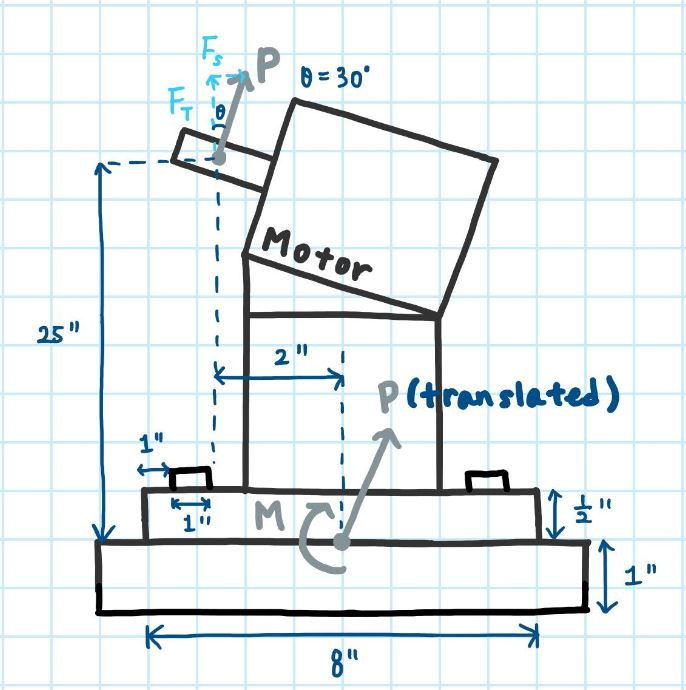
\includegraphics[width=8cm]{BoltForces.jpg}
    \caption{Motor Shaft Force Analysis}
\end{figure}
\noindent From the previous assignment, we know that the force on the motor shaft is the chain tension $P$, where
\begin{center}
    $P$ = 32.01 lbs. Then, by geometry\\
    $F_{T}$ = $P$cos(30) and $F_{S}$ = $P$sin(30)
\end{center}
To calculate the forces affecting the bolts mounted on the plates, we translated $P$ with a representative moment, $M$.
The magnitude of $M$ is given by,
\begin{center}
 $F_{T, \text{total}}$ 
    $M$ = 2$F_{T}$ + 25$F_{S}$
\end{center}

\noindent Since the bolts have to achieve equilibrium with the moment applied by the eccentric load, there must be an extra tensile force on the closest bolts to the shaft, and an extra compressive force on the farther bolts from the shaft. Since the compressive force decreases the load and the tensile force increases the load, the most critical bolts are the two bolts closer to the motor shaft.\\\\
\noindent Therefore if there are four bolts in total, the total tensile and shear forces on each of the bolts are
\begin{center}
   $F_{T,\text{total}} = \dfrac{F_{T}}{4} + \dfrac{M}{4(2.5)}$\\
   $F_{S,\text{total}} = \dfrac{F_{S}}{4}$
\end{center}
where 2.5 is the distance from the centre of a bolt to the middle of the plate since it is recommended that bolts are placed at least its diameter away from the edge of the plate. 

\subsubsection{Stiffness Factors}
To calculate the fraction of external load on the bolts, C, we first found the stiffness factors $k_{b}$ and $k_{m}$. We calculated those as follows

\begin{align*}
    k _ { b } &= \dfrac { A _ { d } A _ { t } E } { A _ { d } l _ { t } + A _ { t } l _ { d } }
    = 12.325 \text{ Mlbf/in} 
\end{align*}

\noindent For the member configuration we note that all the components (washer, top/bottom plate) are made of steel in our system. Therefore, we can calculate the stiffness factor by the following equation:
\begin{equation*}
    k _ { m } = \dfrac { \pi E d \tan \alpha } { 2 \ln \dfrac { \left( l \tan \alpha + d _ { w } - d \right) \left( d _ { w } + d \right) } { \left( l \tan \alpha + d _ { w } + d \right) \left( d _ { w } - d \right) } }
\end{equation*}
Where $l$ is the total thickness of the member configuration, 1.665 in. Since our washer has an outer diameter of 2.5 in while our bolt has a nominal major diameter of 1.0 in, we see that we can substitute $d_w = 2.5d$. We then obtain:
\begin{equation*}
    k _ { m } = \dfrac { 0.5774 \pi E d } { 2 \ln \left( \dfrac{3.5}{1.5} \dfrac { 0.5774 l + 1.5 d } { 0.5774 l + 3.5 d } \right) } = 10.8(10^7) \text{ lbf/in}
\end{equation*}

\noindent We notice that our stiffness for the member a magnitude higher than the stiffness for the bolt. This may be because we are using the same material for all components for our motor mount.\\\\
We are now able to find $C$, the fraction of the external load carried by the bolt:
\begin{align*}
    C = \dfrac { k _ { b } } { k _ { b } + k _ { m } } = 0.103
\end{align*}

\subsubsection{Pre-tension}
Pre-tension is an important aspect of the bolt system since it holds the bolt system together. Shigley's recommends that bolt preload be about 75\% of bolt proof strength in the case that we want to be able to take apart the structure. Since it is important to be able to take apart the structure for maintenance work on the chain (as per last assignment design), we went with a lower estimate of 60\% for extra safety.
\begin{align*}
    F_i &= 0.6S_pA_t\\
    &= 30.9 \text{ kips}
\end{align*}

\subsubsection{Static Calculations}

We then calculated for bolt overload failures in static situations. First, we looked at how close our bolt stresses are to the proof strength. This is described quantitatively by the yielding factor of safety against the static stress exceeding the proof stress and is given by 
\begin{align*}
    n _ { p } &= \dfrac { S _ { p } } { \sigma _ { b } } = \dfrac { S _ { p } A _ { t } } { C F_{T,\text{total}} + F _ { i } } = 1.66
\end{align*}

\noindent While our value is under 2.5, it is still considered a safe design. Shigley's recommends that this safety factor be not much greater than unity for an effective bolt design. This is because the pretension in the bolt is a function of proof strength and area, meaning we are making the pretension be a certain fraction of the bolt proof load to effectively use the bolt strength. Since the pretension in the bolt is orders of magnitude larger than the external load, $n_p$ will be controlled by the pretension, and getting a stronger or larger bolt will not result in any change to this safety factor if we were to use the bolt strength effectively.
\\\\
\noindent Next, we calculate the load factor, which guards against overloading the bolt. This is given by
\begin{align*}
    n _ { L } = \dfrac { S _ { p } A _ { t } - F _ { i } } { C F_{T,\text{total}} } = 4049.8
\end{align*}

\noindent Finally, we calculate factor of safety against joint separation to ensure that the external load does not cause our bolt system to fall apart. This is given by
\begin{align*}
    n _ { 0 } = \dfrac { F _ { i } } { F_{T,\text{total}} ( 1 - C ) } = 695
\end{align*}

\subsubsection{Fatigue Calculations}
To calculate the alternating stress and the midrange stress on the bolts, we use the value of C and $F_{i}$ from the static calculations. 
In this case, our external load alternates between 0 and $F_{T,\text{total}}$. Hence, the maximum alternating stress experienced by a bolt is
\begin{center}
    $\sigma _ { a } = \dfrac { C ( F _ { T,\text{total}})  } { 2 A _ { t } } = 4.12 \text{ psi}$
\end{center}
And the midrange stress is
\begin{center}
    $\sigma _ { \mathrm { m } } = \dfrac { C( F_{T, \text{total}}) } { 2 A _ { t } } + \dfrac { F _ { i } } { A _ { t } } = 51.0 \text{ ksi}$
\end{center}
To calculate the fatigue factor of safety, we used the Goodman criteria. Since it is linear, it is the most conservative and would therefore lead to the safest design. Therefore, the fatigue factor of safety is
\begin{center}
    $n _ { f } = \dfrac { S _ { e } \left( S _ { u t } - \sigma _ { i } \right) } { S _ { u t } \sigma _ { a } + S _ { e } \left( \sigma _ { m } - \sigma _ { i } \right) }$ = 2547.8\\
    \bigskip
    where $\sigma_i = \dfrac{F_{i}}{A_{t}}$
\end{center}
which is beyond our design safety factor of 10.
\subsubsection{Bearing Stress Calculations}
Bearing calculations were performed on both the most critical bolt and the members. The following equation was used to calculate the bearing stress acting on both the bolt and members. 
\begin{equation*}
    \sigma = \dfrac{F}{2td} = \dfrac{27.72}{2(0.5+1)(1)} = 9.24 \text{ lbs/in$^2$}
\end{equation*}
Where $F$ is the shear force acting along the plane, $t$ is the total thickness of the top and bottom plate, and $d$ is the major diameter of the bolt. Note that the top and bottom mounting members are treated as one material from our assumption in the summary section.\\\\
We then obtain our safety factors for both the bolt and member from the following equation:
\begin{align*}
    n_{\text{b}} &= \dfrac{S_p}{\sigma} = \dfrac{85000}{9.24} = 9198.6\\
    n_{\text{m}} &= \dfrac{(S_y)_{\text{mem}}}{\sigma} = \dfrac{45000}{9.24} = 4869.9
\end{align*}
Though we see that both safety factors are very high, they show our system will not reach the Proof Strength of the bolt or the Yield Strength of the material due to bearing stress during its lifetime. Therefore, we can be sure that our system will not fail due to bearing stress on the most critical bolt and/or members.

\subsubsection{Shear Stress Calculations}
Shear calculations were again performed on both the most critical bolt and members. For the shearing stress calculations, it was found that our bolt had threads in the shear plane, defined to be at the location where the top and bottom motor mount plates come into contact. Therefore, we use the following equation:
\begin{equation*}
    \tau_{\text{b}} = \dfrac{F}{4A_r} = \dfrac{27.72}{4(0.551)} = 12.58 \text{ lbs/in$^2$}
\end{equation*}
For our members, we can calculate the shearing stress using:
\begin{equation*}
    \tau_{\text{m}} = \dfrac{F}{4ad} = \dfrac{27.72}{4(1)(1)} = 6.93 \text{ lbs/in$^2$}
\end{equation*}
Here we use $d$ instead of $t$ as shown in the textbook since we know that the plane at which the shear force acts along is correspondent to the area found using the diameter of the bolt its displacement from the edge of the plate.\\\\
We then obtain the following safety factors:
\begin{align*}
    n_{\text{b}} &= \dfrac{0.577S_p}{\tau_{\text{b}}} = \dfrac{0.577(85000)}{12.58} = 3899.3\\
    n_{\text{m}} &= \dfrac{0.577(S_y)_{\text{mem}}}{\tau_{\text{m}}} = \dfrac{0.577(45000)}{6.93} = 3746.6
\end{align*}
As before, we see that both safety factors are very high, and therefore our system will not reach the Proof Strength of the bolt or the Yield Strength of the material due to shear stress and therefore will not fail due to this criterion.

\subsection{Performance Metric}

The total cost of our system, which includes shaft material, shaft machining, bearings, retaining ring grooves, and bolts is \$213.46 as seen in the summary. The total volume of the machined shaft is 278.34 cm$^3$, which weighs 2.19 kg. The weight of the bearings was approximated by the weight of two 30 mm deep groove bearings from \cite{bearings} (0.15 kg each). The total weight is 2.50 kg. The performance metric is calculated with a cost $c$ in dollars as a mass $m$ in kilograms as:
\begin{equation*}
    \text{Performance Metric} = \frac{1}{cm} = \frac{1}{(\$ 213.46)(2.50 \text{ kg})} = 0.00187 \text{ [kg}\cdot\text{\$]}^{-1}
\end{equation*}

\begin{thebibliography}{9}
\bibitem{shigley}
Budynas, Richard G, J K. Nisbett, and Joseph E. Shigley. Shigley's Mechanical Engineering Design. New York: McGraw-Hill, 2011. Print. 

\bibitem{rr}
\textit{MSH Shaft Rings}. Rotor Clip, \url{www.rotorclip.com/cat_pdfs/msh.pdf}.

\bibitem{bearings}
\textit{Deep Groove Ball Bearings}. GMN,\\ \url{www.gmn.de/en/ball-bearings/standard-bearings/groove-ball-bearings/}.
\end{thebibliography}

\end{document}
